\osoba{Mateusz Kempa}

\zadanieprojektowe{Przegląd aplikacji open source}{2015-10-29}{2015-10-31}{zakończone}

Poszukiwania aplikacji open source wykorzystujących GPS rozpocząłem na dwóch najpopularniejszych serwisach z otwartymi oraz darmowymi apkami na platformę Android tj., {\color{blue}\underline{\href{https://f-droid.org/repository/browse/?fdcategory=Navigation}{F-Droid}}} oraz {\color{blue}\underline{\href{https://fossdroid.com/c/navigation/whats_new.html}{Fossdroid}}}. Na tych witrynach znajduje się multum narzędzi open source służących do nawigacji w systemie Android. Niestety, wymagań projektowych nie spełnia żadne z nich. Wtedy z pomocą przyszedł Google Play. Aplikacja, którą tam znalazłem nazywa się \textbf{WayPoint} i wydaję się być przydatna z mojego punktu widzenia. Po otwarciu, WayPoint szuka sygnału GPS i jeżeli nasze urządzenie złapie fixa, można zapisać aktualne współrzędne lokalizacji, w której się znajdujemy - Add WayPoint. Kiedy już zapisaliśmy punkt(y), wybieramy żądany z menu My WayPoints. W tym momencie przechodzimy już do nawigacji. Aplikacja oblicza odległość dzielącą nas od celu oraz wyświetla jego współrzędne. Do wyboru mamy widok mapy lub wskaźnika. To wszystko. Choć opisana aplikacja jest dość prosta to można moim zdaniem wykorzystać ją do projektu. Na pewno nie obędzie się bez modyfikacji. Poniżej zamieszczam parę screenshotów oraz link do repozytorium.

\begin{figure}[H]
\centering
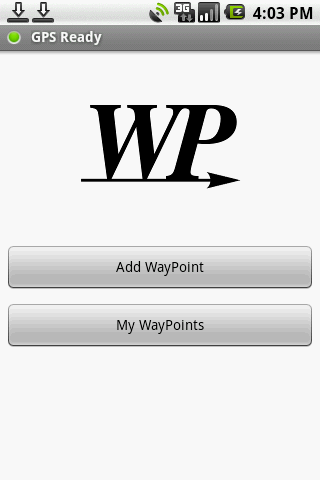
\includegraphics[scale=0.5]{czlonkowie/3/1waypoint.png}
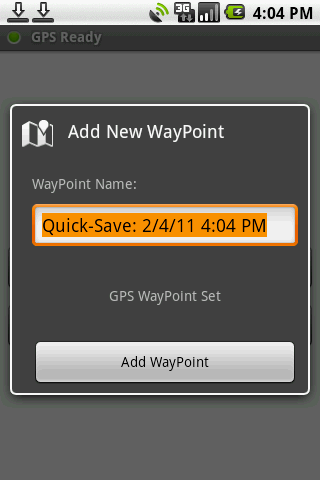
\includegraphics[scale=0.5]{czlonkowie/3/2waypoint.png}
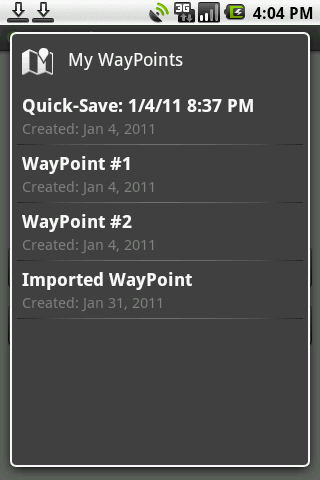
\includegraphics[scale=0.5]{czlonkowie/3/3waypoint.png}
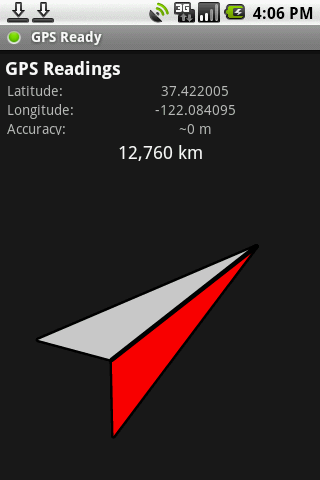
\includegraphics[scale=0.5]{czlonkowie/3/4waypoint.png}
\end{figure}

Repozytorium: {\color{blue}\underline{\href{https://github.com/pettyjamesm/WayPoint}{github.com/pettyjamesm/WayPoint}}}
\newline \newline
Inne aplikacje open source warte uwagi: {\color{blue}\underline{\href{https://github.com/andreynovikov/Androzic}{Androzic}}}, {\color{blue}\underline{\href{https://github.com/borneq/HereGPSLocation}{HereGPSLocation}}}

\zadanieprojektowe{Przeanalizowanie aplikacji Waypoint i określenie w jakim stopniu będzie pomocna przy projekcie}{12.11.2015} {16.11.2015}{zakończone} 

\zadanieprojektowe{Wyszukiwanie uszkodzonych kodów kreskowych}{03.12.2015}{05.12.2015}{zakończone}

Podczas pierwszej wizyty w czytelni, naszym zadaniem było naklejanie części kodów kreskowych na regałach. Niestety, po naklejeniu okazało się, że niektóre kody zostały przez nieuwagę zatarte. Mogło to w przyszłości spowodować problemy z odczytem. Do moich obowiązków należało odnalezienie uszkodzonych kodów kreskowych, spisanie ich, przygotwanie gotowego do druku pliku pdf zgodnego z wymaganiami projektowymi. W czasie pierwszego spotkania projektowego w czytelni, kody kreskowe zostały naklejone na 40 regałach.

\zadanieprojektowe{Naklejanie kodów kreskowych na regałach  w czytelni}{28.11.2015}{05.12.2015}{zakończone}

Tym razem podzieliliśmy zakres obowiązków między wycinanie i naklejanie kodów oraz naklejanie folii ochronnej. Do mnie należało naklejanie kodów kreskowych oraz folii. Zdołaliśmy nakleić kody na regały 40-90. Przy wycinaniu wystąpił pewien problem i niektóre kody kreskowe uległy nie mogły zostać naklejone. Konieczne było ich spisanie, aby można było je następnym razem uzupełnić.

\zadanieprojektowe{Naklejanie kodów kreskowych na regałach w czytelni c.d.}{08.12.2015}{12.12.2015}{zakończone}

Na tym spotkaniu naszym celem było naklejenie pozostałych kodów łącznie ze wcześniej uszkodzonymi oraz zabezpieczenie ich folią. Podział obowiązków był jednak większy, gdyż tylko 2 osoby mogły się tym razem stawić w czytelni. Ja zająłem się przygotowaniem folii oraz naklejeniem części kodów. Po ukończeniu naszych zadań wszystkie kody na 102 regałach były gotowe do użycia.  

\zadanieprojektowe{Edycja dokumentacji}{08.12.2015}{}{w realizacji} 

Na podstawie przykładowej dokumentacji, zmodyfikowałem sekcje: "Cele nowego projektu" oraz "Zakres nowego projektu".

\zadanieprojektowe{Odczyt kodów kreskowych z książek}{15.12.2015}{}{w realizacji} 

Odczytaliśmy kody z książek z pierwszych 20 regałów. Moim zadaniem była kontrola odczytu i zapisu kodów kreskowych w notatniku.










